%\RequirePackage{lineno}
\documentclass[aps,prc,preprint,superscriptaddress,showpacs,showkeys]{revtex4-1}
\usepackage{graphicx}

\begin{document}
%\linenumbers
\title{{\Large Quarkonia suppressions in PbPb collisions at $\sqrt s_{NN}$ =  2.76 TeV }}
\author{\large Vineet Kumar}
\author{\large Prashant Shukla}
\email{pshukla@barc.gov.in}
\affiliation{Nuclear Physics Division, Bhabha Atomic Research Center, Mumbai, India}
\affiliation{Homi Bhabha National Institute, Anushakti Nagar, Mumbai, India}
\date{\today}


\begin{abstract}
 We calculate the $J/\psi$ and $\Upsilon$ suppression and regeneration assuming quark gluon plasma
produced in PbPb collisions at LHC energy. The quarkonia suppression is estimated using well knowen 
process of gluon dissociation in medium. The rate of regeneration has been obtained 
using principle of detailed balance and is compared with that obtained using statistical hadronization 
model. The suppression factors due to cold nuclear matter effects 
have been obtained from measurements of quarkonia in pPb collisions.
  The nuclear modification factor as a function of centrality and transverse momentum has been calculated  
and compared to J/$\psi$ and $\Upsilon$ nuclear modification factors measured in PbPb collisions 
at $\sqrt s_{NN}$ =  2.76 TeV.
\end{abstract}

\pacs{12.38.Mh, 24.85.+p, 25.75.-q}
\keywords{quark-gluon plasma, quarkonia, suppression, regeneration}
\maketitle


%%%%%%%%%%%%%%%%%%%%%%%%%%%%%%%%%%%%%%%%%%%%%%%%%%%%%%%%%%%%%%%%%%%%%%%%%%%%%%%%%%%%%%%%%%
\section{Introduction}
   The heavy ion collisions produce matter at extreme temperatures and densities where 
it is expected to be in the form of Quark Gluon Plasma 
(QGP), a phase in which the quarks and gluons can move far beyond  the size of a nucleon 
making colour degrees of freedom dominant in the medium. 
  The experimental effort to produce such matter started with low energy CERN accelerator 
SPS and evolved through voluminous results from heavy ion collision at Relativistic Heavy Ion 
Collider (RHIC) \cite{INTRO}.
 The recent results from Large Hadron Collider (LHC) experiments \cite{QGP_Tc} are 
pointing towards formation of high temperature system in many ways similar to the matter
produced at RHIC. 
  One of the most important signal of QGP is the suppression of 
quarkonium states \cite{SATZ}, both of the charmonium ($J/\psi$, $\psi(2S)$, $\chi_{c}$, etc) 
and the bottomonium ($\Upsilon(1S)$ , $\Upsilon(2S)$, $\chi_{b}$, etc) families. This is thought to be a 
direct effect of deconfinement, when the binding potential between the constituents of a quarkonium state, 
a heavy quark and its antiquark, is screened by the colour charges of the surrounding light quarks and gluons. 
  The ATLAS and CMS experiments have carried out detailed quarkonia measurements in Pb+Pb collisions 
with the higher energy and luminosity available at the LHC.
 The ATLAS measurements \cite{ATLAS} show suppression of inclusive $J/\psi$ with high transverse momenta $p_T$  
in central PbPb collisions compared to peripheral collisions at $\sqrt s_{NN} = 2.76$ TeV. 
  Similarly, CMS measured a steady and smooth decrease of suppression 
of prompt $J/\psi$ as a function of centrality with nuclear modification factor $R_{AA}$ remaining $<$ 1 even 
in the peripheral bin \cite{JCMS,CMSJPsi}. ALICE shows that low p$_T$ J/$\psi$ are less suppressed and show very 
little centrality dependence\cite{ALICEJPsi}.
  The melting temperature of the quarkonia states depend on their binding energy. The ground states, 
$J/\psi$ and $\Upsilon(1S)$ are expected to dissolve at significantly higher temperatures than the 
more loosely bound excited states. 
   The $\Upsilon(2S)$ and $\Upsilon(3S)$ have smaller binding energies as compared to ground
state $\Upsilon(1S)$ and hence are expected to dissolve at a lower temperature. 
 With the 2011 Pb+Pb run the CMS published results on sequential suppression of 
$\Upsilon(nS)$ states as a function of centrality \cite{CMSU2} with enlarged statistics
over their first measurement \cite{UCMS}, where a suppression of the excited $\Upsilon$ states with respect 
to the ground state have been observed  
in PbPb collisions compared to pp collisions at $\sqrt s_{NN} = 2.76$ TeV \cite{YSuppAbdShuk}.
  The quarkonia yields in heavy ion collisions are also modified due to non-QGP effects such as
shadowing, an effect due to change of the parton distribution functions inside the nucleus,
and dissociation due to nuclear or comover interaction \cite{Vogt}.
  If large number of heavy quarks are produced in initial heavy ion collisions at LHC energy 
this could even lead to enhancement of quarkonia via statistical recombination \cite{Rapp1,Rapp2,Andronic_SH}. 

 In this paper, we calculate the charmonia suppression due to thermal gluon dissociation in an expanding
Quark Gluon Plasma. Other sources which can alter the yield of charmonium are considered 
e.g. nuclear shadowing and comover interaction. 
We also consider the effect of J/$\psi$ regeneration using the statistical hadronization model.
J/$\psi$ yield is studied as a function of impact parameter or centerality of events. 
Calculations are compared with experimental data from CMS and ALICE.


\section{Heavy quark production rates}
The production cross sections for heavy quark pairs are calculated to NLO in pQCD  
using the CTEQ6M parton densities \cite{CTEQ6}.  The central EPS09 parameter set 
\cite{EPS09} is used to calculate the modifications of the parton densities in 
Pb+Pb collisions.  We use the same set of parameters
as that of Ref.~\cite{CNV} with the NLO calculation of Ref.~\cite{MNR}
to obtain the exclusive $Q \overline Q$ pair rates as well as their decays
to dileptons.  
 The production cross sections for heavy flavor and quarkonia at $\sqrt{s_{_{NN}}}= 2.76$ 
TeV \cite{ContinuumVKShuk} are given in Table~\ref{NLOcros}.  The number of $Q \overline Q$ pairs
in a minimum bias Pb+Pb event is obtained from the per nucleon cross
section, $\sigma_{\rm PbPb}$, by
\begin{eqnarray}
N_{Q \overline Q} = {A^2 \sigma_{\rm PbPb}^{Q \overline Q}  \over  
\sigma_{\rm PbPb}^{\rm tot}} \, \, .
\end{eqnarray}
 At 2.76 TeV, the total Pb+Pb cross section, $\sigma_{\rm PbPb}^{\rm tot}$, 
is 7.65 b \cite{PbPbTotal}.

\begin{table}
\caption[]{Heavy quark and quarkonia cross sections at
$\sqrt{s_{_{NN}}}= 2.76$ TeV. The cross sections are given per nucleon while
$N$ gives number of heavy quark pair/quarkonia per Pb+Pb event.}
\label{NLOcros}
\begin{tabular}{l|l|l|l|l} 
\hline 
\hline
                     & $ c \overline c$           &J/$\psi$      & $ b \overline b$           & $\Upsilon$   \\              
\hline
$\sigma_{\rm PbPb}$  & $1.76^{+2.32}_{-1.29}$ mb  & $31.4 \mu$b  & $89.3^{+42.7}_{-27.2}$ mb  & $0.38 \mu$b  \\
$N$                  &$9.95^{+13.10}_{-7.30}$     & $0.177$      & $0.50^{+0.25}_{-0.15}$     & $0.01$       \\
\hline
\hline
\end{tabular}
\end{table}


\begin{table}
\caption[]{Quarkonia properties as predicted by non-relativistic potential model using 
``Cornell'' potential\cite{YSuppAbdShuk}.}
\label{QuarkoniaProperties}
\begin{tabular}{l|l|l|l|l|l|l|l|l} 
\hline   
\hline
    &J/$\psi$  &$\chi_c$  &$\psi(2S)$ &$\Upsilon(1S)$ &$\chi_b(1P)$ &$\Upsilon(2S)$ &$\chi_b(2P)$ &$\Upsilon(3S)$ \\ 
\hline 
Mass [GeV/$c^2$]                      &3.10     &3.53  &3.68  &9.46  &9.99  &10.02  &10.26   &10.36 \\
Binding Energy [GeV]                  &0.64     &0.20  &0.05  &1.10  &0.67  &0.54   &0.31    &0.20 \\
Radius [fm]                            &0.25     &0.36  &0.45  &0.14  &0.22  &0.28   &0.34    &0.39 \\
Formation time $\tau_{\rm Form}$ [fm]  &0.89     &2.0   &1.5   &0.76  &2.6   &1.9    &2.6      &2.4 \\
\hline
\hline
\end{tabular}
\end{table}




%%%%%%%%%%%%%%%%%%%%%%%%%%%%%%%%%%%%%%%%%%%%%%%%%%%%%%%%%%%%%%%%%%%%%%%%%%%%%%%%%%%%%%%%%%


\section{Modification of quarkonia in presence of QGP}

  The number of quarkonia $N(\tau_0,p_T)$ produced at initial time $\tau_0$ is modified due to 
dissociation in the medium and thus the number at freeze out time $\tau_f$ can be written as  
\begin{equation}
N(\tau_f,p_T) = S(p_T) \,N(\tau_0,p_T).
\label{eqbeta}
\end{equation}
The survival probability $S(p_T)$ of quarkonia from gluon dissociation is given as 
\begin{equation}
S(p_T) = \exp \left( {-\int_{\tau_0}^{\tau_f}\Theta(\tau-\tau_{\rm{F}})f(\tau)\lambda_{\rm D}(T)\,\rho_g(T)\,d\tau} \right), 
\end{equation}
where $\tau_{\rm{F}} = \tau_{\rm Form~}p_T/M$ in terms of formation time $\tau_{\rm Form}$
of quarkonium state, $\rho_g(T)$ is the gluon density of QGP at temperature $T$.
 We use vacuum formation time, $\tau_{\rm Form}$ 0.87 fm (0.76 fm) for J/$\psi$ ($\Upsilon$)\cite{YSuppAbdShuk}.     
$\tau_f$ is the freezeout time. Other properties of quarkonia are given in Table~\ref{QuarkoniaProperties}.
f$(\tau)$ repersent the QGP fraction at proper time $\tau$.  
The dissociation rate $\lambda_D$ is obtained by averaging the dissociation cross section over the 
gluon momentum distribution as follows
\begin{equation}
\lambda_{\rm D}(T)=\langle \sigma_D v_{\mathrm{rel}} \rangle.
\label{LamdaDRhod}
\end{equation}


  The nuclear modification factor ($R_{AA}$) can be written as 
\begin{equation}
R_{AA}(N_{\rm part}) = \frac{\int_{p_{Tmin}}^{p_{Tmax}} N(\tau_0,p_T)S(p_T)dp_T}{\int_{p_{Tmin}}^{p_{Tmax}} N(\tau_0,p_T) dp_T}
\label{raa}
\end{equation}
 The $R_{AA}$ including the regenration can be written as 
\begin{equation}
R_{AA} = S(p_T) + N_{J/\psi}^{\rm Regen}.
\end{equation}
where $N_{J/\psi}^{\rm Regen}$ is number of J/$\psi$s per event produced from uncorrelated pairs of 
Q$\overline{Q}$ at the time of hadronization as explained in section \ref{SHM}. 

\begin{figure}
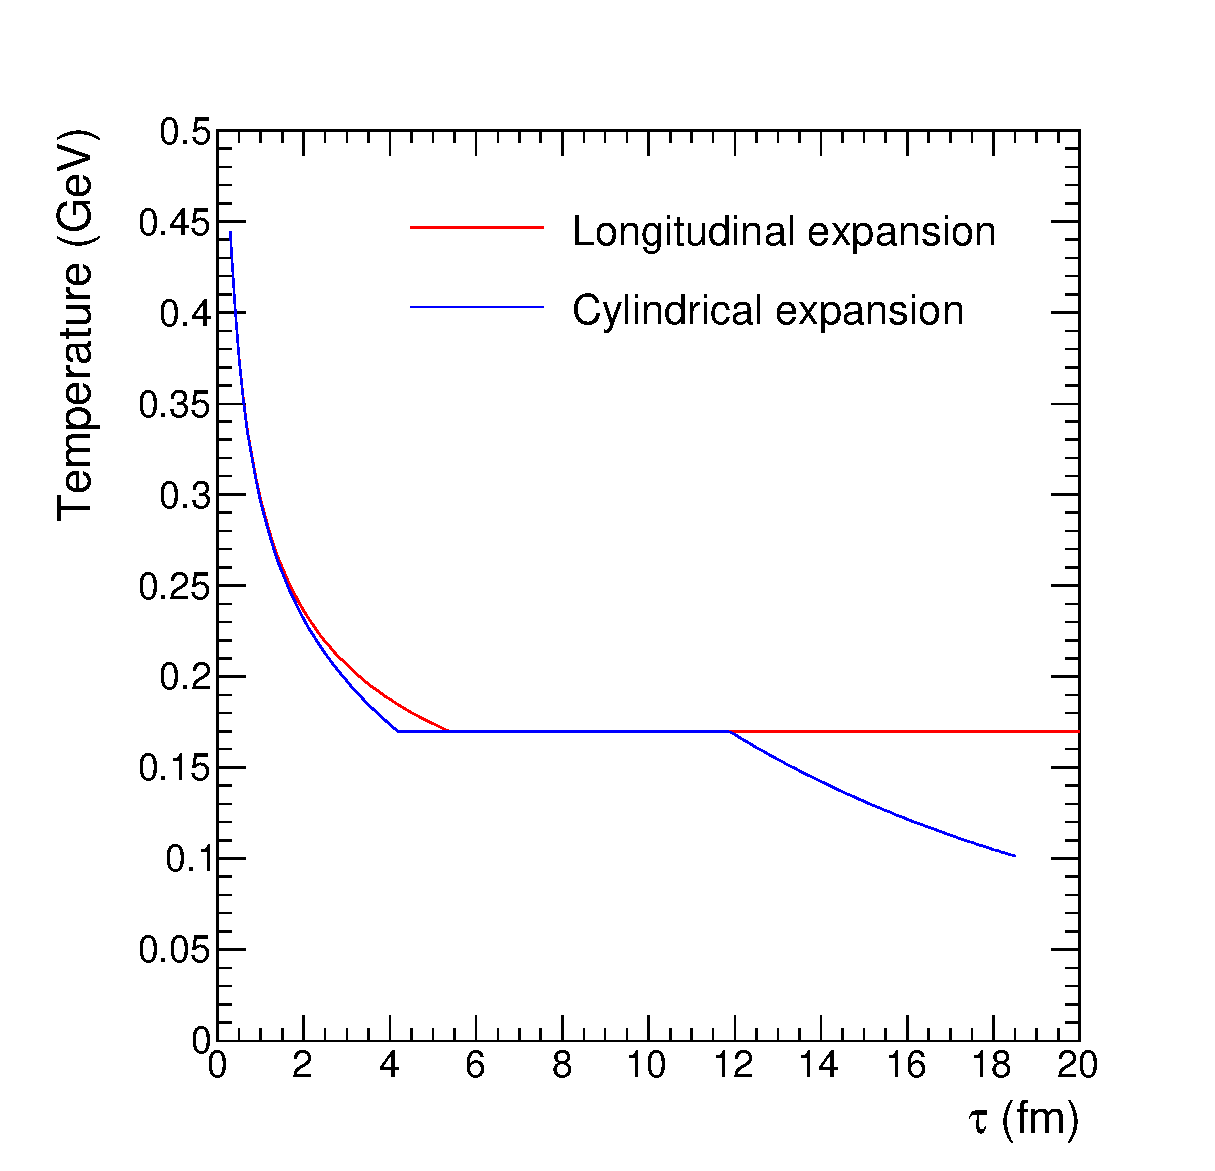
\includegraphics[width=0.60\textwidth]{Fig1_TauVsTemp.eps}
\caption{(Color online) Temperature of the system as a function of proper time in case of 
longitudinal expansion and cylindrical expansions.}
\label{fig:TauVsTemp}
\end{figure}



 The temperature evolution for different centralities of collision is obtained by 
assuming an isentropical cylindrical expansion with volume element
\begin{equation}
V(\tau) = \tau\,\pi\,(r_0 + {1\over 2} a \, \tau^2 )^{2}\Delta y,
\end{equation}
 where a$_T$=0.1c$^2$ fm$^{-1}$ is the transverse acceleration \cite{RAPc}.
 The initial transverse radius, $r_0$ as a function of centrality is 
obtained in terms of the radius of the Pb nucleus ($R_{0}$) as
\begin{equation}
r_0(N_{\rm part}) = R_0 \, \sqrt{N_{\rm part} \over N_{\rm part0} }.
\label{RVsNPart}
\end{equation}
where $N_{\rm part0} = 2A$ is the total number of participants in head on collisions.

The temperature variation with time is obtained by  
\begin{eqnarray}
s(\tau)\,V(\tau)= s(\tau_0)\,V(\tau_0)=S. 
\end{eqnarray}
Using $s(\tau)=4a_qT^3$ 
\begin{eqnarray}
T(\tau)^{3} = \frac{S}{4a_qV(\tau)}.
\end{eqnarray}
where $a_{q} = (7N_f/60 + 16/90)\pi^2$ is the degrees of freedom in quark gluon phase.
We relate initial temperature with measured charged particle multiplicity as
\begin{eqnarray}
S = 4a_qV(\tau_0)|_{0-5\%} T_{0}^{3} =3.6\left(\frac{dN}{d\eta}\right)_{0-5\%}. 
\label{TempVsMult}
\end{eqnarray}  
Using $(dN/d\eta)_{0-5\%}$=1.5$\times$1600 obtained from the charge particle multiplicity measured in 
Pb+Pb collisions at 2.76 TeV \cite{MULT} and N$_f$ = 2.5, we calculate initial temperature
0.641 GeV at time $\tau_0$ = 0.1 fm/c.
Transverse size of the system for 0-5$\%$ centrality is $R_{0-5\%}$ = 0.92$R_0$,
 obtained from Eq.~(\ref{RVsNPart}). 
The initial temperature for different centralities is calculated by 
\begin{equation}
T_{0}^{3}({N_{\rm part}})=T_{0}^{3}\left(\frac{dN/d\eta}{N_{\rm part}/2}\right)/\left(\frac{dN/d\eta}{N_{\rm part}/2}\right)_{0-5\%}
\label{TempNpart}
\end{equation}




%%%%%%%%%%%%%%%%%%%%%%%%%%%%%%%%%%%%%%%%%%%%%%%%%%%%%%%%%%%%%%%%%%%%%%%%%%%%%%%%%%%%%%%%%%%%%%%%%

\begin{figure}
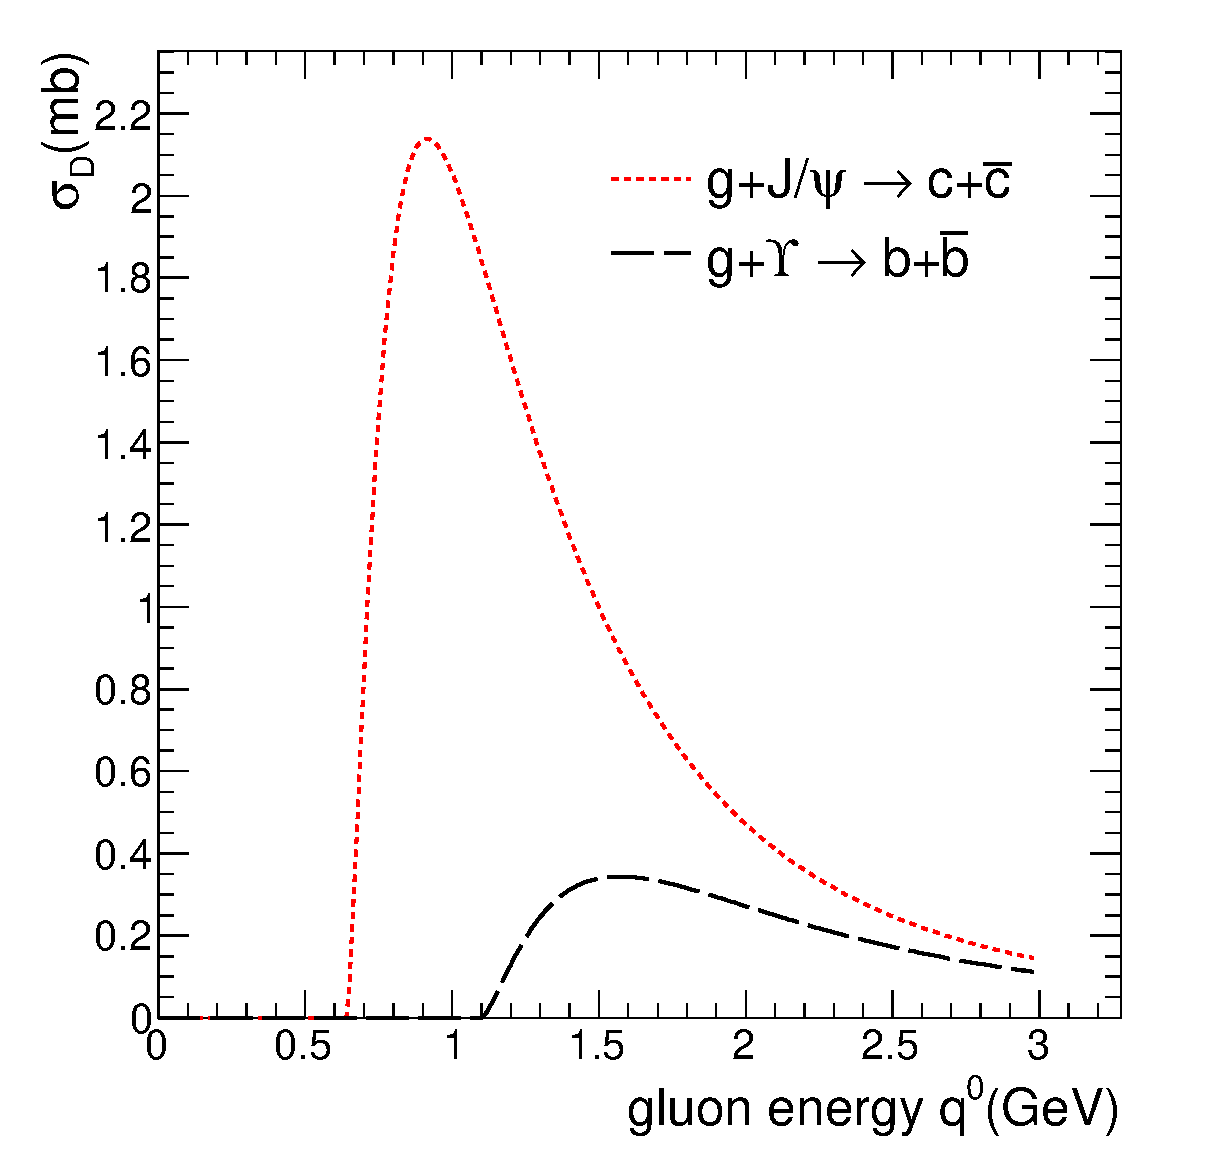
\includegraphics[width=0.60\textwidth]{Fig2_SigmaDq0.eps}
\caption{Cross section for gluon dissociation of quarkonia as a function of gluon energy $q^{0}$ in
quarkonia rest frame.}
\label{fig:SigmaDQ0}
\end{figure}

\begin{figure}
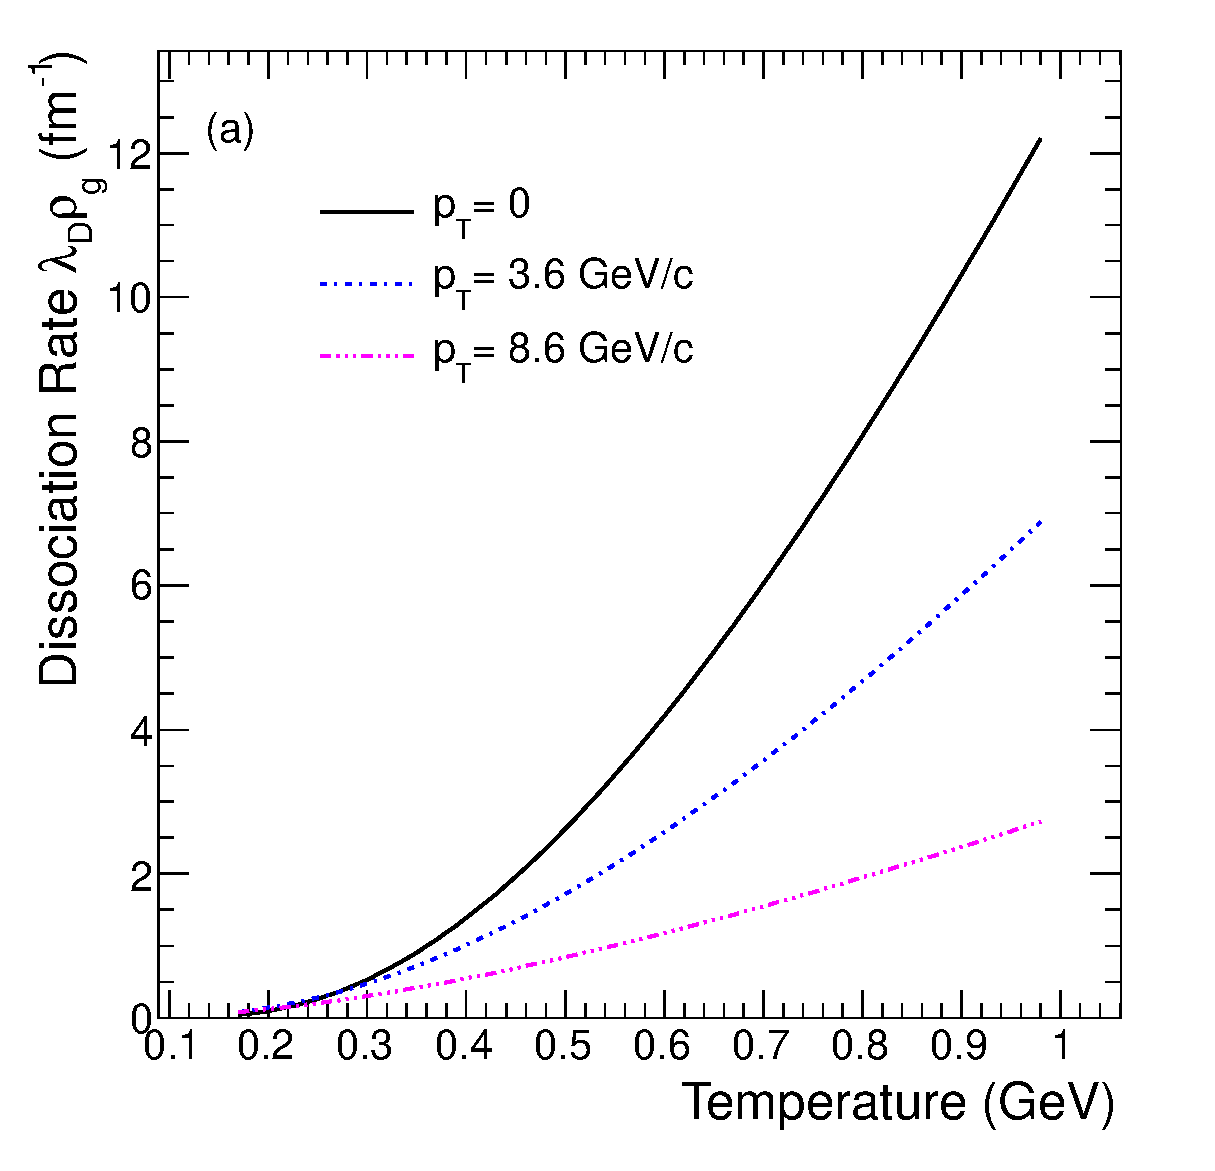
\includegraphics[width=0.49\textwidth]{Fig3a_DRateVsT.eps}
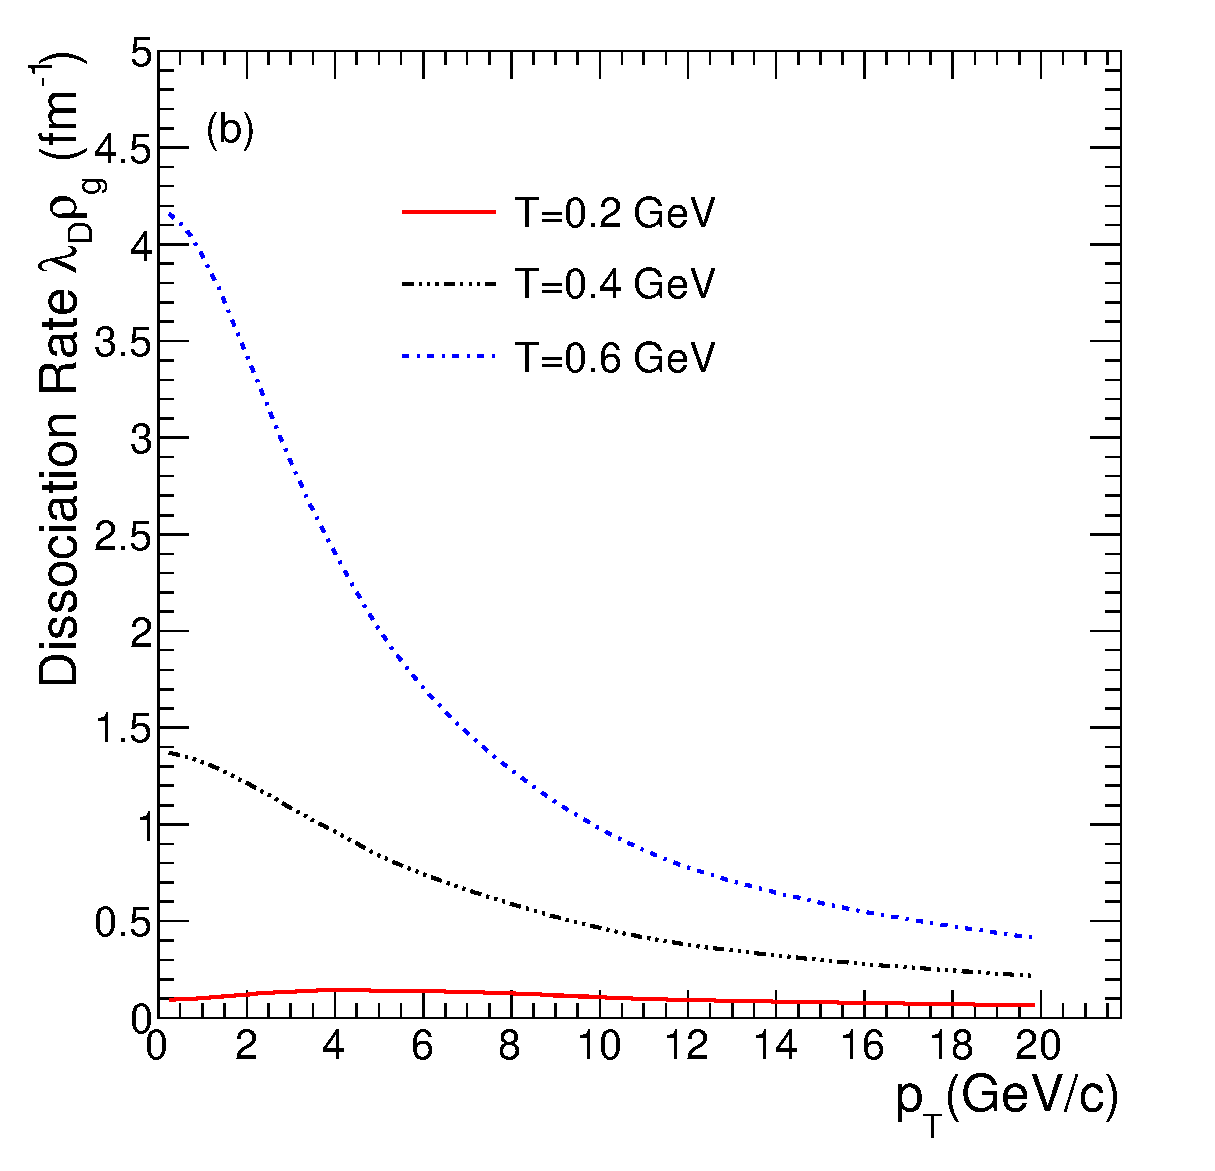
\includegraphics[width=0.49\textwidth]{Fig3b_DRateVsPt.eps}
\caption{(Color online )Variation of dissociation rate with a) temperature and with b) transverse momentum.}
\label{fig:DRateVsTempAndPt}
\end{figure}


\section{Dissociation Rate}
The gluon-$J/\psi$ dissociation cross section in dipole approximation is given by \cite{ks95}

\begin{equation}
\sigma_{D}(q^{0}) = 4\pi\,\left(\frac{8}{3}\right)^3\,\frac{1}{m_Q^{3/2}}\,\epsilon_0^3 \frac{ (q^0-\epsilon_0)^{3/2}}{(q^0)^5}
\end{equation}
where $m_Q$ is the heavy quark mass, and $q^0$ the gluon energy in the $J/ \psi$ rest
frame; its value must be larger than the $J/\psi$ binding energy
$\epsilon_0$. 

\begin{eqnarray}
\langle \sigma v \rangle &= & \frac{1}{(2\pi)^{3}} \int d^{3}p_{g} f_{g}(p_{g},T) v_{\rm rel} \sigma_{D}(s) \\ \nonumber
 				      &= &\frac{1}{(2\pi)^{3}} \int  2\pi p_{g}^{2} dp_{g} f_{g}(p_{g},T) \int \sigma_{D}(s) v_{\rm rel}(s) \theta(s-\Delta E_{Q}^{2}) d(cos\theta) 
\end{eqnarray}
 
 If we consider that the $J/ \psi$ moves in the transverse direction with a four-velocity
$u=(M_T, \vec{P_T}, 0)/M_{J/\psi}$, where $M_T=\sqrt{p_T^2+M^2_{J/ \psi}}$ is defined as the $J/\psi$'s
transverse mass. A gluon with a four-momentum $k=(k^0,\vec{k})$
in the rest frame of the parton gas has an energy $q^0=k\cdot u$
in the rest frame of the $J/\psi$ given by
\begin{eqnarray}
 q^{0} &= &\frac{k^{0}\,m_{T} + \vec{k} \cdot \vec{p_{T}}}{M_{J/\psi}}, \nonumber \\
       &= &\frac{s-M_{J/\psi}^{2}}{2\,M_{J/\psi}},
\end{eqnarray}
The dissociation rate is given by 
\begin{eqnarray}
\lambda_D = \langle v_{\rm rel} \sigma_{D} (k \cdot u)\rangle_k &= &\frac{\int d^3k v_{\rm rel} \sigma_{D} (k \cdot u) f(k^0,T)}{\int d^3k f(k^0,T)},
 \label{eq5}
\end{eqnarray}
where the gluon distribution in the rest frame of the parton gas is
\begin{equation}
  f(k^0,T)=\frac{\lambda_g(=16)}{e^{k^0/T}-1} \label{eq6}.
\end{equation}
The relative velocity $v_{\rm rel}$ between the $J/\psi$ and a gluon is
\begin{eqnarray}
 v_{\rm rel}  =  \frac{P_{J/\psi}\cdot k}{k^0M_T} \,\,
              =  1-\frac{\vec{k}\cdot\vec{P}_T}{k^0M_T} \,\,
              =  {s- M_{J/\psi} \over 2E_1E_2}  
\label{eq7}
\end{eqnarray}


  Changing the variable to the gluon momentum, $q=(q^0,\vec{q})$, in
the rest frame of the $J/\psi$, and writing $\rho_g = \int d^3k f(k^0,T)$, 
the Eq.~(\ref{eq5}) can be rewritten as
\begin{eqnarray}
\lambda_D \rho_g  =  \int d^3q \frac{M_{J/\psi}}{m_T}\sigma_{D}(q^0) f(k^0,T).
\label{eq8}
\end{eqnarray}
  Using $ k^0=(q^0M_T+\vec{q}\cdot\vec{P}_T)/M_{J/\psi}$ in Eq.~\ref{eq8} and solving
\begin{eqnarray} 
\lambda_D\,\rho_g &= &\frac{M_{J/\psi}}{m_T} \int d^3q \, \sigma_{D}(q^0) \frac{\lambda_{g}} {  e^{ \frac{q^0m_{T}}{M_{J/\psi}T}} e^{ \frac{ \vec{q}\cdot \vec{p_{T} } }{ M_{J/\psi}T }  } -1}  \nonumber \\
%&= &\frac{\lambda_{g}}{2\pi^3} \frac{M_{J/\psi}}{m_T} \int d^3q \, \sigma_{D}(q^0)   \sum_{n=1}^{\infty}  e^{ \frac{-n\,q^0 m_{T}}{M_{J/\psi}T}} e^{  \frac{-n\,\vec{q}\cdot \vec{p_{T}}}{M_{J/\psi}T}}  \nonumber \\
%&= &\frac{\lambda_{g}}{2\pi^3} \frac{M_{J/\psi}}{m_T}  \sum_{n=1}^{\infty} 2\pi  \int (q^0)^2 dq^0 \, \sigma_{D}(q^0)\,e^{ \frac{-n\,q^0m_{T}}{M_{J/\psi}T}}  \int_{1}^{-1} e^{  \frac{-n\,q^0\,p_{T} cos\theta}{M_{J/\psi}T}} d(cos\theta) \nonumber \\
%&= &\frac{\lambda_{g}}{2\pi^3} \frac{M_{J/\psi}}{m_T} \sum_{n=1}^{\infty} 2\pi  \int (q^0)^2 dq^0 \, \sigma_{D}(q^0)\,e^{ \frac{-n\,q^0 m_{T}}{M_{J/\psi}T}} 
%    \left[ e^{-\frac{nq^0 p_T}{M_{J/\psi}T}} - e^{\frac{nq^0 p_T}{M_{J/\psi}T}} \right]\,\frac{M_{J/\psi}T}{nq^0 p_T}  \nonumber \\
&= &\frac{\lambda_{g}}{2\pi^3} \frac{M_{J/\psi}^2}{m_T} 2\pi \sum_{n=1}^{\infty} \frac{T}{n} \int_{\epsilon_0}^{\infty} q^0 dq^0 \, \sigma_{D}(q^0)  
     \,e^{ \frac{-n\,q^0 m_{T}}{M_{J/\psi}T}} 
     \frac{1}{p_T} \left[e^{\frac{n q^0 p_T}{M_{J/\psi}T}} - e^{- \frac{n q^0 p_T}{M_{J/\psi}T}}\right] \\ \nonumber
\label{dissrate}
\end{eqnarray}


% The special case of Eq.~(\ref{dissrate}) for J/$\psi \,p_T = 0$ is
%\begin{eqnarray} 
%  \frac{1}{p_T} \left[e^{\frac{n q^0 p_T}{M_{J/\psi}T}} - e^{- \frac{n q^0 p_T}{M_{J/\psi}T}}\right] = {2nq^0\over M_{J/\psi}T}.
%\label{case}
%\end{eqnarray}
%Using this we get 
%\begin{eqnarray} 
% \lambda_D\,\rho_g &= &  4\pi \int (q^0)^2\,dq^0 \, \sigma_{D}(q^0) \frac{\lambda_{g}} {e^{\frac{q^0}{T}} -1}
%\end{eqnarray}




%%%%%%%%%%%%%%%%%%%%%%%%%%%%%%%%%%%%%%%%%%%%%%%%%%%%%%%%%%%%%%%%%%%%%%%%%%%%%%%%%%%%
%\section{Formation Rate}
%  We can calculate formation rate from dissociation rate using detailed balance relation \cite{THEWF} 
%\begin{equation}
% \sigma_{F} = \frac{48}{30}\,\sigma_{D}(q^0)\frac{(s-M_{J/\psi})^{2}}{s(s-4m_{c}^{2})}.
%\end{equation}
%The formation rate can be written as 

%\begin{equation}
%\lambda_{F} = <\sigma_{F} \,\, v_{\rm rel}>
%\end{equation}
%v$_{\rm rel}$ is relative velocity between c $\bar{c}$ quark pair and is given by

%\begin{eqnarray}
%v_{\rm rel} &=& {\sqrt{(p_{1}.p_{2})^{2} - m_Q^{4} } \over E_{1} \, E_{2}} \nonumber \\
%            &=& \frac{\sqrt{s(s-4m_{Q}^{2})}}{2E_1E_2}.
%\end{eqnarray}
%Here
%\begin{eqnarray}
% s &= &(E_1+E_2)^{2} - (\vec{p_1}+\vec{p_2})^2 \nonumber \\
%   &= & m_Q^{2} + m_Q^{2} + 2 E_1E_2 - 2 |\vec{p_1}||\vec{p_2}|cos\theta 
%\end{eqnarray}
%where $\vec{p_{1}}$ and $\vec{p_{2}}$ are three momentum of quarks. 

%The final expression for formation rate can be written as
%\begin{eqnarray}
%\lambda_{F} &= &\frac{\int \sigma_{F}(s)\, v_{\rm rel}\,f_{c}(p_1)\, f_{\bar{c}} (p_2) \,d^{3}p_1 \,d^{3}p_2} {\int \,f_{c}(p_1)\,d^{3}p_1 \,\, \int f_{\bar{c}} (p_2)\,d^{3}p_2}\\
%            &= &\frac{\int \sigma_{F}(s)\, v_{\rm rel}\,f_{c}(p_1)\, f_{\bar{c}} (p_2) \, 4\pi p_1^{2} dp_1 \, 2\pi p_2^{2} dp_2 d(cos \theta)}
%           {4\pi \int p_1^{2} dp_1 \,f_{c}(p_1) \,\, 4 \pi \int p_2^{2} dp_2 \, f_{\bar{c}} (p_2)}.
%\end{eqnarray}
%and $f_{c}(p)$ and $f_{\bar{c}}(p)$ are parton distribution function of c and $\bar{c}$ respectively and are given by
%\begin{equation}
%f_{c}(p)={g_c(=6)  \over 1 + {\rm exp} [ { (p^{2} + m^{2} )^{1/2}  \over T }] }.
%\end{equation}

%\begin{figure}
%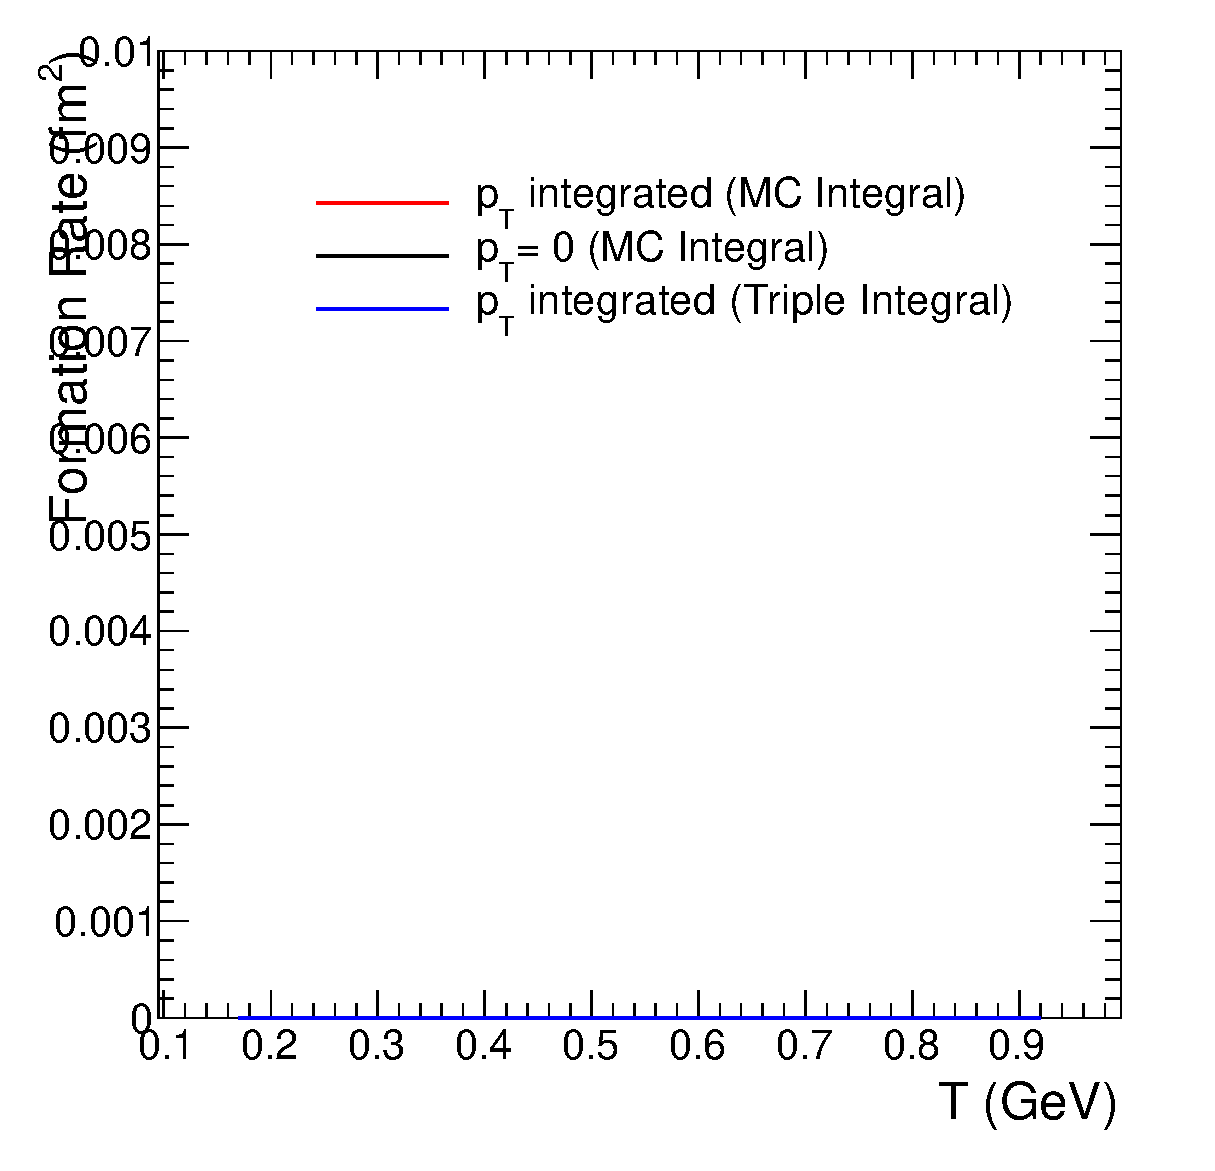
\includegraphics[width=0.48\textwidth]{FormRateVsT.eps}
%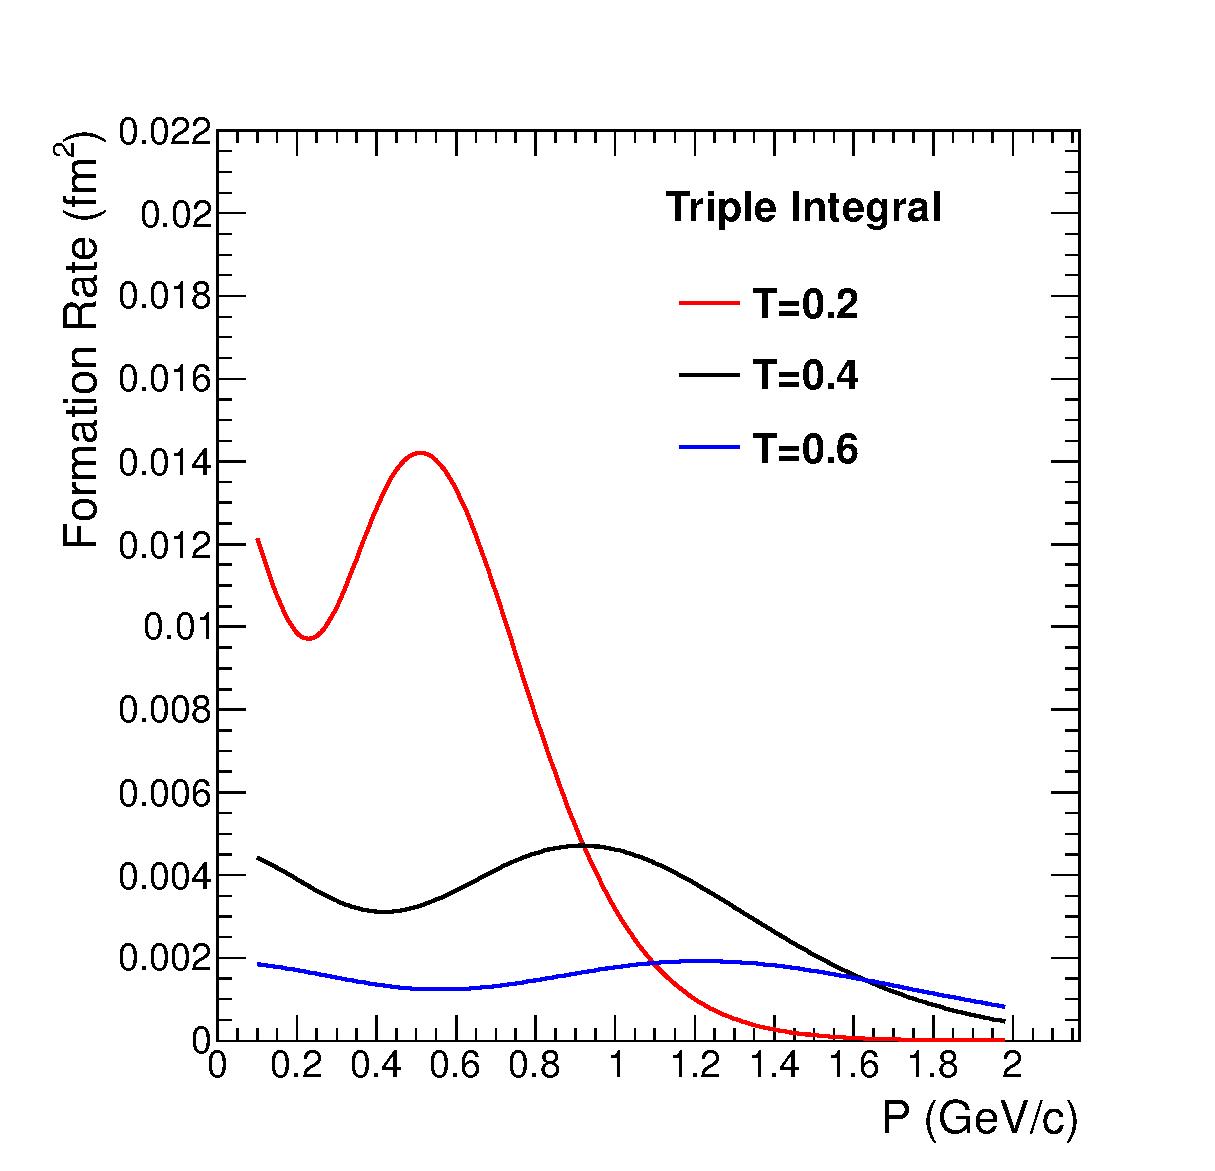
\includegraphics[width=0.48\textwidth]{FormRate_TriInt.eps}
%\caption{(Color online) Formation rate as a function of (a) temperature and (b) transverse momentum.}
%\label{fig:ForRateVsTempAndPt}
%\end{figure}

%%%%%%%%%%%%%%%%%%%%%%%%%%%%%%%%%%%%%%%%%%%%%%%%%%%%%%%%%%%%%%%%%%%%%%%%%%%%%%%%%%%%%%



\section{Formation of quarkonia  by statistical hadronization model}\label{SHM}
The heavy quark production at LHC is substantial which may lead to incoherent 
recombination of uncorrelated pairs of heavy quarks and anti quarks which result 
from multiple pair production. In statistical approach \cite{MUNZI} the number of 
J/$\psi$ produced is given by 
\begin{eqnarray}
N_{J/\psi}  &= &4 {n_{ch} n_{J/\psi} \over n_{\rm open}^2}  {N_{c\bar c}^2 \over N_{ch} }\\
          &= &\frac{N_{c\overline{c}}^{2}}{V}\frac{4n_{J/\psi}}{n_{open}^{2}}.
\end{eqnarray}
where $n_i$'s are the thermal densities, $N_{c\bar c}$ is the number of charm pairs produced 
and $N_{ch}$ is the number of total charged particle produced. 
The freeze out parameters are $T=170$ MeV and $\mu_B = 0$. For
$dN_{ch}/dy = 1600$ \cite{MULT} and $dN_{c \bar c} /dy = 14.0$, we obtain $dN_{J/\psi} /dy = 0.0092$.
The densities can be calculated using thermal distributions of various particles.

\begin{equation}
n_{open} = {4\pi \,g_{D} \over (2\pi)^{3}} \int_{0}^{\infty} f_{D}(p)p^{2}dp
\end{equation}
by the same method we can calculate the J/$\psi$ number density as

\begin{equation}
n_{J/\psi} = {4\pi \,g_{J/\psi} \over (2\pi)^{3}} \int_{0}^{\infty} f_{J/\psi}(p)p^{2}dp 
\end{equation}
 For total charge particle density we can use 

\begin{equation}
n_{ch} = 2 \,n_{\pi} + 2\, n_{K} + 2\, n_{p},
\end{equation}
where
\begin{equation}
n_{\pi} = {4\pi \,g_{\pi} \over (2\pi)^{3}} \int_{0}^{\infty} f_{\pi}(p)p^{2}dp.
\end{equation}

 The J/$\psi$ generated from recombination of uncorrelated heavy quark pairs will have 
softer $p_{T}$ distributions than that of J/$\psi$ coming from initial hard scattering and thus 
effect of recombination will be important only at low $p_T$. We consider the contributions of recombined J/$\psi$
only for low $p_{T}$ measurements made by ALICE detector as shown in Fig. \ref{fig:JPsiRaa} (a).     
 We do not consider effect of recombination for high $p_{T}$ measurement made by CMS detector \cite{CMSUpsilon,CMSJPsi} 
as shown in Fig. \ref{fig:JPsiRaa} (b). As production cross section of bottom quark is small even at LHC energies,
we do not consider effect of recombination for $\Upsilon$ measurement shown in Fig. \ref{fig:UpsilonRaa}(c).



\begin{figure}
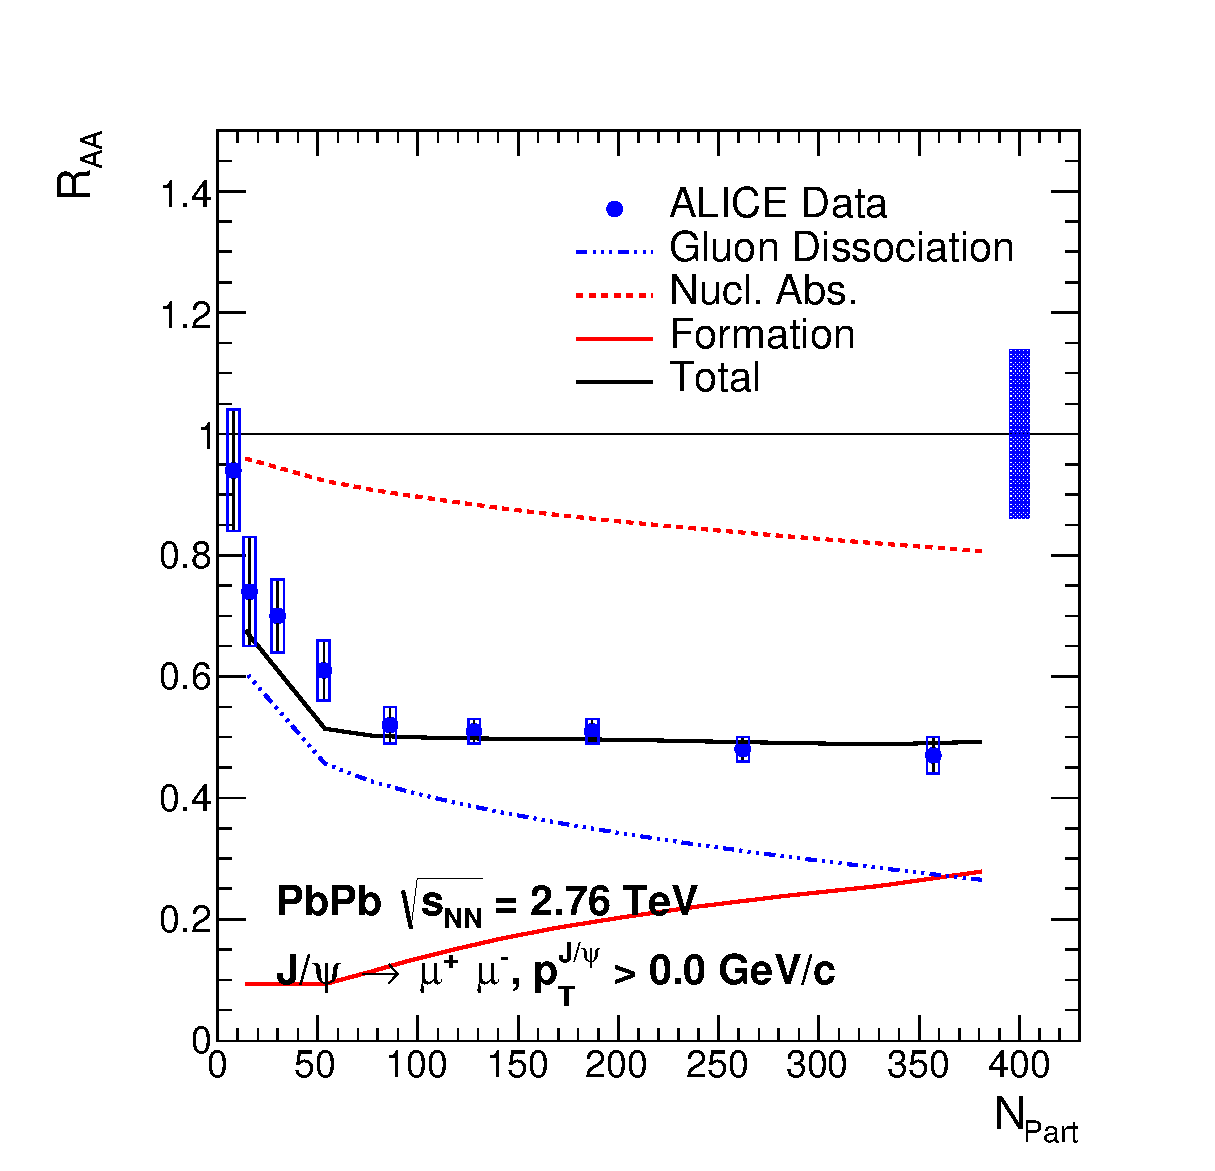
\includegraphics[width=0.49\textwidth]{Fig4a_ALICE_RAA.eps}
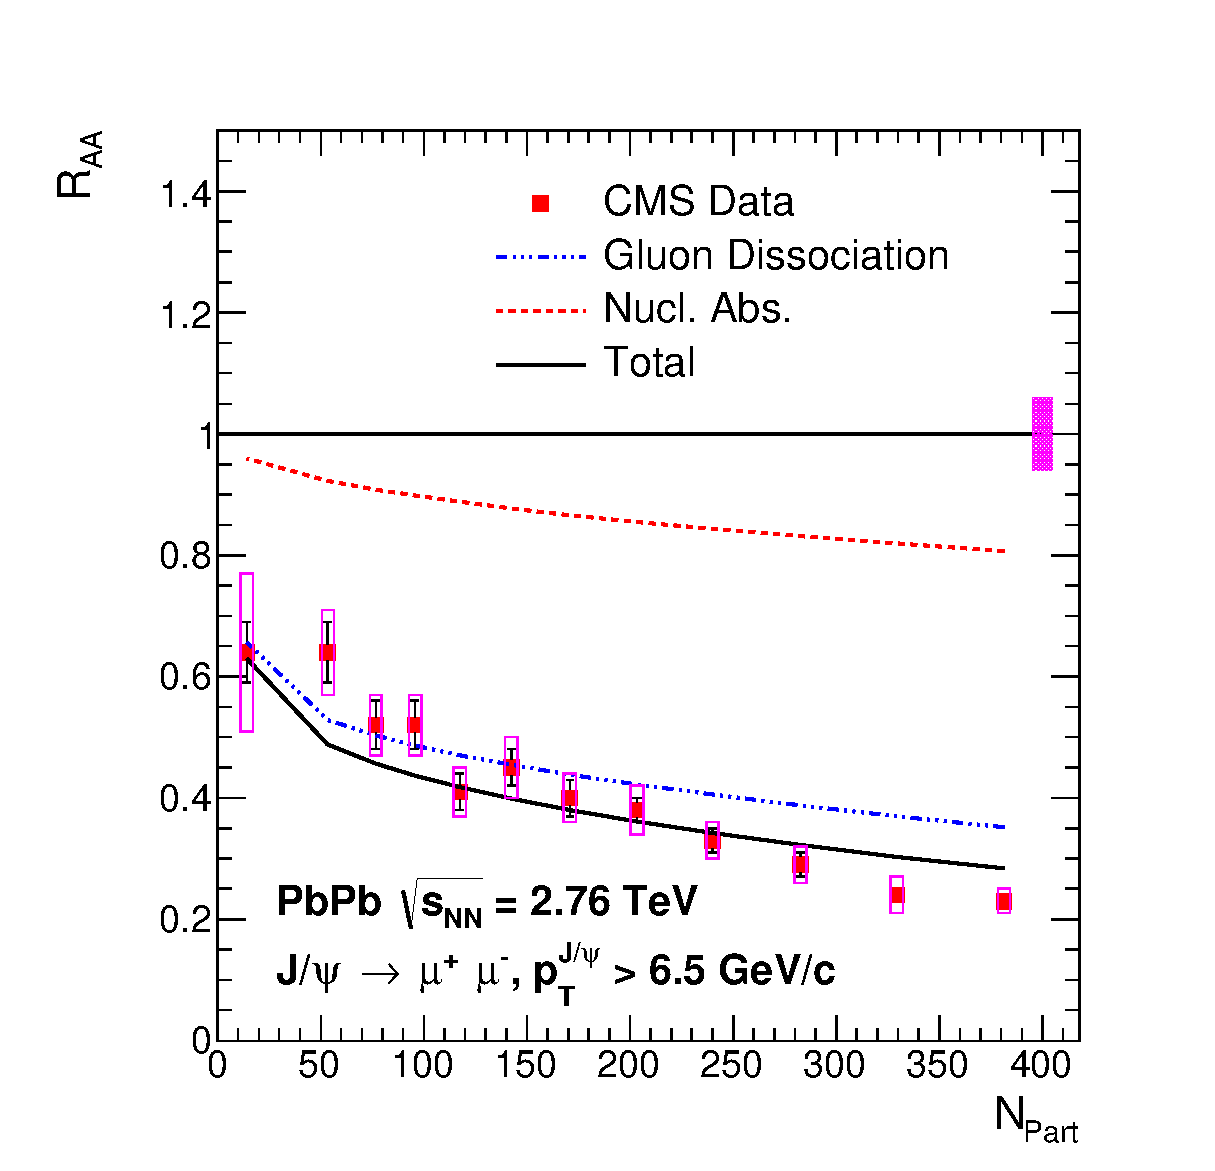
\includegraphics[width=0.49\textwidth]{Fig4b_CMS_RAA_JPsi.eps}
\caption{(Color online) Nuclear modification factor (R$_{AA}$) compared with ALICE and CMS data.}
\label{fig:JPsiRaa}
\end{figure}

\begin{figure}
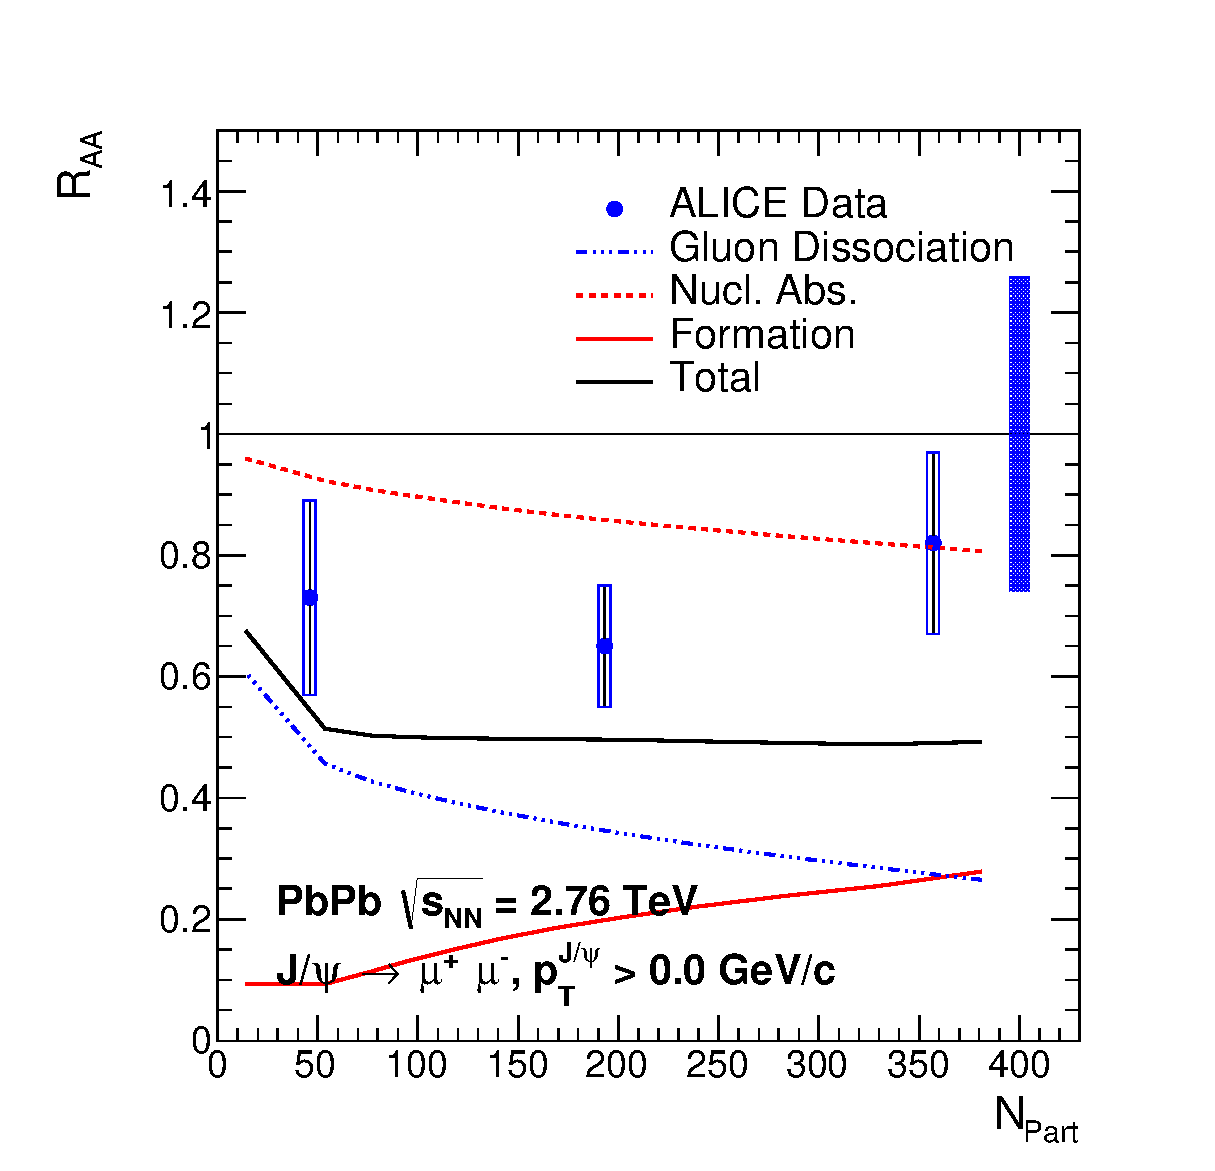
\includegraphics[width=0.60\textwidth]{Fig5_ALICEMid_RAA.eps}
\caption{(Color online) Nuclear modification factor (R$_{AA}$) compared with ALICE data at mid
rapidity.}
\label{fig:JPsiRaaALICEMid}
\end{figure}

\begin{figure}
\includegraphics[width=0.49\textwidth]{Fig6a_CMS_RAA_Upsilon.eps}
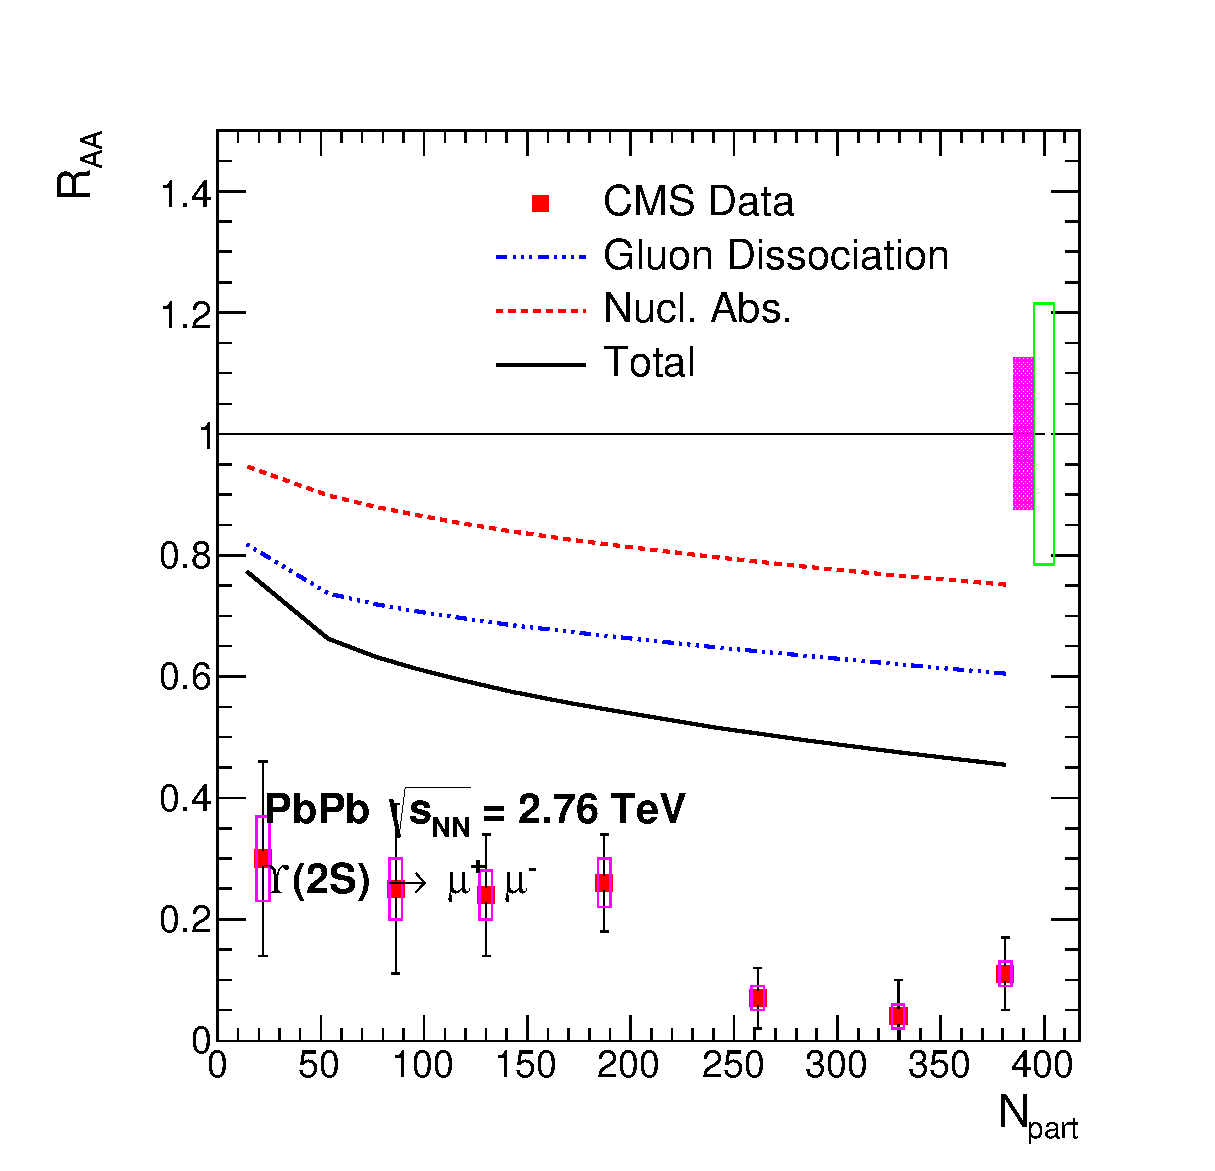
\includegraphics[width=0.49\textwidth]{Fig6b_CMS_RAA_Upsilon2S.eps}
\caption{(Color online) Nuclear modification factor (R$_{AA}$) compared with CMS $\Upsilon$ data. }
\label{fig:UpsilonRaa}
\end{figure}

%%%%%%%%%%%%%%%%%%%%%%%%%%%%%%%%%%%%%%%%%%%%%%%%%%%%%%%%%%%%%%%%%%%%%%%%%%%%%%%%%%%%%%%%
 
\section{Cold matter effects}
The quarkonia can be suppressed due to cold matter effects such as shadowing and due to nuclear
matter and comover interaction. For simplicity we approximate the combination of all CNM effects 
by a suppression factor,
\begin{equation}
  S_{Nucl}=\exp[-\rho_{N}\sigma_{abs}L(b)]
  \label{CNMF}
\end{equation}
with an effective nuclear absorption cross section, $\sigma_{abs}$.
We take absorption cross section, $\sigma_{abs}$ = 3 mb (2 mb) for
J/$\psi$($\Upsilon$). The other parameters in Eq. \ref{CNMF} are the nuclear density,
$\rho_N$=0.14 fm$^{-3}$, and the impact-parameter dependent path length, L(b), evaluated 
with a Glauber model \cite{GM_PShukla} for the nuclear overlap.


%%%%%%%%%%%%%%%%%%%%%%%%%%%%%%%%%%%%%%%%%%%%%%%%%%%%%%%%%%%%%%%%%%%%%%%%%%%%%%%%%%%%%%%




\section{Summary}

 The $J/\psi$ and $\Upsilon$ modification in medium are calculated and compared to the data
measured by CMS and ALICE.
  The $J/\psi$ suppression is estimated using process of gluon dissociation in medium. The rate of regeneration 
has been obtained using principle of detailed balance and is compared with that obtained using statistical 
hadronization model. 
 The suppression factors due to cold nuclear matter effects 
have been obtained from measurements of quarkonia in pPb collisions.
 The nuclear modification factor as a function of centrality and transverse momentum has been calculated  
and compared to J/$\psi$ and $\Upsilon$ nuclear modification factors measured in PbPb collisions 
at $\sqrt s_{NN}$ =  2.76 TeV.
  Our model with both, gluon dissociation and nuclear absorption describes the data very well although, 
slight difference in most central collisions may be due to reduction of binding energy of quarkonia with temperature 
and lowering of quark mass.



\noindent
\begin{thebibliography}{100}
\medskip
\bibitem{INTRO} I. Arsene {\it et al.} [BRAHMS Collaboration], Nucl. Phys. A {\bf 757}, 1 (2005); 
  B.B. Back {\it et al.} [PHOBOS Collaboration], Nucl. Phys. A {\bf 757} 28.(2005); 
  J. Adams {\it et al.} [STAR Collaboration], Nucl. Phys. A {\bf 757}, 10.(2005); 
  K. Adcox {\it et al.} [PHENIX Collaboration], Nucl. Phys. A {\bf 757} 184 (2005).
\bibitem{QGP_Tc} B. Muller, J. Schukraft and B. Wyslouch, Ann. Rev. Nucl. Part. Sci., arXiv:1202.3233 [hep-ex].
\bibitem{SATZ} T. Matsui and H. Satz, Phys. Lett. B{\bf 178}, 416 (1986).
\bibitem{ATLAS} G. Aad {\it et al.} [ATLAS Collaboration], Phys. Lett. B{\bf 697},294 (2011); arXiv:1012.5419.
\bibitem{JCMS} S. Chatrchyan {\it et al.} [CMS Collaboration] J. High Energy Phys. {\bf 1205}, 63 (2012);  arXiv: 1201.5069 [nucl-ex]..
\bibitem{CMSJPsi} Camelia Minrov (for the CMS Collaboration) Nucl. Phys. A {\bf 904} 194 (2013).
\bibitem{ALICEJPsi} Enrico Scomparin (for the ALICE Collaboration) Nucl. Phys. A {\bf 904} 202 (2013).
\bibitem{CMSU2} CMS Collaboration, CERN-PH-EP-2012-228, arXiv:1208.2826.
\bibitem{UCMS} S. Chatrchyan {\it et al.} [CMS Collaboration] Phys. Rev. Lett. {\bf 107}, 052302 (2011).
\bibitem{YSuppAbdShuk} A. Abdulasalam and P. Shukla, arXiv:1210.7584.
\bibitem{Vogt} R. Vogt, Phys. Rev. C{\bf 81}, 044903 (2010); arXiv:1003.3497.
\bibitem{Rapp1} X. Zhao and R. Rapp, Nucl. Phys. A{\bf 859}, 114 (2011); arXiv:1102.2194. 
\bibitem{Rapp2} X. Zhao and R. Rapp, Phys. Rev. C{\bf 82}, 064905 (2010); arXiv:1008.5328.
\bibitem{Andronic_SH} A. Andronic, P. Braun-Munzinger, K. Redlich, J. Stachel Nucl. Phys. A {\bf 905} 535 (2013); arXiv:1210.7724.
\bibitem{CTEQ6} J.~Pumplin, D.~R.~Stump, J.~Huston, H.~L.~Lai, P.~M.~Nadolsky 
and W.~K.~Tung,  JHEP {\bf 0207}, 012 (2002) [arXiv:hep-ph/0201195];
  D.~Stump, J.~Huston, J.~Pumplin, W.~K.~Tung, H.~L.~Lai, S.~Kuhlmann  and J.~F.~Owens,
  JHEP {\bf 0310}, 046 (2003)  [arXiv:hep-ph/0303013].
\bibitem{EPS09} K. J. Eskola, H. Paukkunen and C. A. Salgado, JHEP{\bf 0904}, 065 (2009) [arXiv:0902.4154 [hep-ph]].
\bibitem{CNV} M. Cacciari, P. Nason and R. Vogt, Phys. Rev. Lett.{\bf 95}, 122001 (2005).
\bibitem{MNR} M. L. Mangano, P. Nason, and G. Ridolfi, Nucl. Phys. B{\bf 373}, 295 (1992).

\bibitem{ContinuumVKShuk} V. Kumar, P. Shukla and R. Vogt, Phys. Rev. C{\bf 86}, 054907 (2012).

\bibitem{PbPbTotal} Total PbPb

\bibitem{RAPc} Rapp 

%\bibitem{THEWS} R. L. Thews and J. Rafalski, Nuclear Physics A698, 575 (2002) [arXiv: hep-ph/0104025];
               R. L. Thews, arXiv: hep-ph/0206179.
%\bibitem{Rapp} R. Rapp, arXiv: hep-ph/xxxx.
%\bibitem{bj83} J. D. Bjorken, Phys. Rev. D{\bf 27}, 140 (1983). 
\bibitem{MULT} K. Aamodt {\it et al.} [ALICE collaboration], Phys. Rev. Lett. {\bf 106}, 032301 (2011);
          arXiv:1012.1657 [nucl-ex].
%\bibitem{CMSmult} S. Chatrchyan {\it et al.} [CMS Collaboration], J. High Energy Phys. {\bf 1108}, 141 (2011);
       arXiv:1107.4800.  
\bibitem{ks95}D.~Kharzeev and H.~Satz, CERN-TH/95-117, BI-TP 95/20,
         {\it Quark-Gluon Plasma II}, R. C. Hwa (Ed.) (World Scientific, Singapore)
%\bibitem{KEXW}K.~J.~Eskola and X.-N.~Wang, Phys. Rev. D {\bf 49}, 1284(1994).
\bibitem{THEWF} R.L. Thews and M.L. Mangano, arXiv:nucl-th/05050552 (2006).
\bibitem{MUNZI} P. Braun-Munzinger and J. Stachel Phys. Lett. B {\bf 490} 196 (2000).
\bibitem{CMSUpsilon} S. Chatrchyan {\it et al.} [CMS Collaboration], Phys. Rev. Lett. {\bf 109} 222301 (2012). 
\bibitem{GM_PShukla} P. Shukla arXiv: nucl-th/0112039. 
\end{thebibliography}
\end{document}
